\documentclass[11pt,a4paper]{article}
\usepackage[utf8]{inputenc}
\usepackage[T1]{fontenc}
\usepackage[english]{babel}
\usepackage{lmodern}
\usepackage[margin=2.5cm]{geometry}
\usepackage{amsmath,amssymb}
\usepackage{graphicx}
\usepackage{booktabs}
\usepackage{tabularx}
\usepackage{caption}
\usepackage{float}
\usepackage{setspace}
\usepackage{microtype}
\usepackage{xcolor}
\usepackage[round,authoryear]{natbib}
\usepackage[colorlinks=true,linkcolor=blue!50!black,citecolor=blue!50!black,urlcolor=blue!50!black]{hyperref}
\captionsetup{font=small,labelfont=bf,justification=centering}
\newcommand{\nota}[1]{\par\vspace{2pt}\begin{minipage}{\linewidth}\footnotesize\textit{Note}: #1\end{minipage}}
\onehalfspacing

\title{\textbf{More Guns, More Homicides? Firearm Deregulation in Brazil and Lethal Violence across Municipalities and the Soy Frontier (2015--2024)}}
\author{Ricardo Alves dos Santos\thanks{Universidade do Estado de Mato Grosso (UNEMAT), Inovapro. Corresponding author. E-mail: \href{mailto:ricardo.alves@unemat.br}{ricardo.alves@unemat.br}.}
\and Cleiton Franco\thanks{Universidade do Estado de Mato Grosso (UNEMAT), Inovapro, Sinop, Brazil.}
\and Wylmor Dalfovo\thanks{Universidade do Estado de Mato Grosso (UNEMAT), Inovapro.}
\and Lindomar Pegorini\thanks{Universidade do Estado de Mato Grosso (UNEMAT), Inovapro.}}
\date{November 2026}

\begin{document}
\maketitle
\thispagestyle{empty}

\begin{abstract}
\noindent Between 2019 and 2022, a sequence of federal decrees relaxed access to firearms in Brazil, and new civilian gun registrations more than doubled. This paper estimates the effect of this expansion on firearm homicides by linking municipal records from the National Firearms System (SINARM) to death records from the Mortality Information System for all 5,570 Brazilian municipalities between 2015 and 2024. Identification exploits municipal variation in the intensity of the shock through difference-in-differences designs with a continuous treatment, staggered adoption \citep{callaway2021}, and synthetic difference-in-differences \citep{arkhangelsky2021}. Each additional registration per 1,000 inhabitants in 2019--2022 raises the firearm homicide rate by @@b2@@ per 100,000, and municipalities that experienced a registration surge record, on average, @@cs@@ additional deaths per 100,000. The effect is confined to firearm deaths, does not appear in knife homicides, and is larger on the soy frontier, where it reaches @@soycs@@ deaths per 100,000. Synthetic difference-in-differences estimates are sensitive to the choice of comparison group, and there is no evidence of reversal after the 2023 restrictions.

\vspace{0.6em}
\noindent\textbf{Keywords}: firearms; homicides; difference-in-differences; synthetic control; agricultural frontier; Brazil.

\noindent\textbf{JEL codes}: K42; I18; C23; R11; Q15.
\end{abstract}

\newpage
\setcounter{page}{1}

\section{Introduction}

Between 2019 and 2022, Brazil went through the deepest change in firearm regulation since the 2003 Disarmament Statute (Law 10,826/2003). A sequence of presidential decrees and Army ordinances relaxed the requirement to demonstrate effective need for civilian gun ownership, raised purchase limits for firearms and ammunition, and extended access to restricted calibers to hunters, sport shooters, and collectors (CACs). The number of active CAC registration certificates rose from 117,467 in 2018 to 783,385 in 2022 \citep{fbsp2023}, and new civilian firearm registrations in SINARM went from about 75 thousand per year in 2018--2019 to 165 thousand in 2021. Decrees 11,366 and 11,615 reversed part of these measures in 2023.

The effect of such an expansion on lethal violence is theoretically ambiguous. In the rational choice model of \citet{becker1968}, a higher probability that victims are armed raises the expected cost of crime and may deter offenders. A larger stock of guns in circulation, however, makes interpersonal conflicts more lethal and facilitates the diversion of firearms to illegal markets. International evidence tends to favor the second channel \citep{duggan2001,cook2006}, and the Brazilian experience with the Disarmament Statute points in the same direction \citep{souza2007,cerqueira2012}. For the recent deregulation cycle, the available evidence is aggregated at the regional or state level \citep{baculi2021,wakim2025} and does not exploit variation across municipalities in the intensity with which the regulatory shock materialized.

This paper estimates the effect of the expansion of gun registrations on firearm homicides in all 5,570 Brazilian municipalities between 2015 and 2024. The exposure measure is built from SINARM open microdata, which record each firearm by municipality, month, and owner category, and outcomes come from the Mortality Information System (SIM). The empirical strategy combines difference-in-differences with a continuous treatment, the staggered-adoption estimator of \citet{callaway2021}, and the synthetic difference-in-differences (SDID) estimator of \citet{arkhangelsky2021}. A triple difference that compares firearm and knife homicides within the same municipality and year isolates the gun-availability channel. The paper also examines the soy frontier, where the recent expansion of planted area coincides with deforestation and a strong demand for armed self-defense, motivated by evidence that soy expansion raised homicides in Brazil \citep{moreno2024}.

The results indicate that deregulation increased firearm homicides. In the main specification, each additional registration per 1,000 inhabitants raises the rate by @@b2@@ deaths per 100,000 per year (standard error @@b2se@@), equivalent to @@iqr@@ deaths per 100,000 when moving from the first to the third quartile of exposure. The \citet{callaway2021} estimator yields an average effect of @@cs@@ deaths per 100,000 in municipalities that experienced a registration surge. The effect is specific to firearm deaths and is larger on the soy frontier (@@soycs@@ per 100,000). Pre-treatment coefficients from the conventional event study are not jointly zero, and SDID estimates depend on the definition of the comparison group; these limitations are discussed in detail.

The paper makes three contributions. First, it provides the first municipal-level causal estimates of the effects of the 2019--2022 deregulation. Second, it builds a reproducible panel that integrates four public data sources (SINARM, SIM, IBGE, and MapBiomas). Third, it applies SDID to the evaluation of gun policy, as recommended by \citet{benmichael2024}, and documents territorial heterogeneity associated with soy expansion. Section~\ref{sec:contexto} describes the policy; Section~\ref{sec:dados} presents the data; Section~\ref{sec:estrategia} discusses the empirical strategy; Sections~\ref{sec:resultados} to \ref{sec:soja} present the results; Section~\ref{sec:conclusao} concludes.

\section{Institutional background}\label{sec:contexto}

The Disarmament Statute made civilian gun ownership conditional on demonstrating effective need, assessed by the Federal Police. Decree 9,685 of January 2019 presumed such need for residents of rural areas and of states with more than 10 homicides per 100,000 inhabitants, a threshold met in practice by every state. Decrees 9,785, 9,845, and 9,846 of 2019 raised ammunition limits and broadened the list of permitted firearms, and Decrees 10,627 to 10,630 of 2021 increased the number of guns allowed per owner. Decree 11,366 of January 2023 and Decree 11,615 of July 2023 reversed part of these measures.

Figure~\ref{fig:mensal} shows the monthly response of registrations. Until 2019, new civilian registrations fluctuated between 4 and 8 thousand per month. The acceleration gained strength from mid-2020, peaked in 2021 at up to 16 thousand registrations per month, and vanished from late 2022 onward, when registrations stabilized at about 2 thousand per month. The lag between the 2019 decrees and the 2020 acceleration indicates that the shock materialized gradually and with different intensity across municipalities, which motivates measuring exposure as the cumulative registrations between 2019 and 2022 and defining cohorts by each municipality's first registration surge.

\begin{figure}[H]
\centering
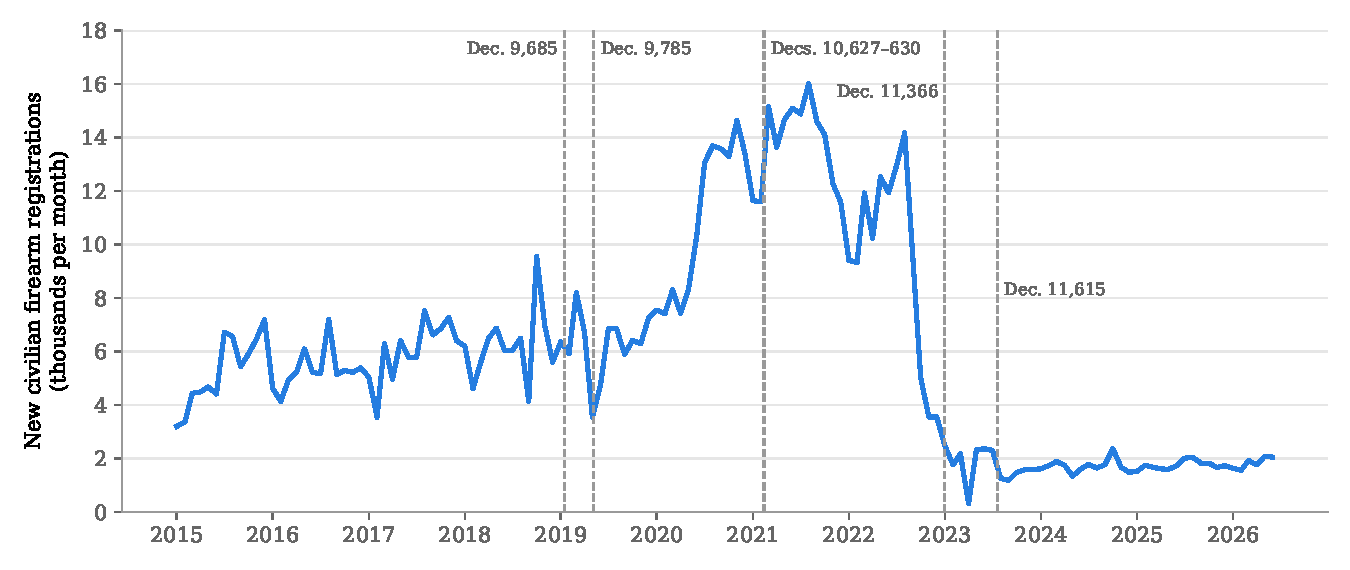
\includegraphics[width=\linewidth]{figs/registros_mensais_en.pdf}
\caption{Monthly new civilian firearm registrations in Brazil and regulatory milestones}\label{fig:mensal}
\nota{National sum of SINARM registrations in the ``Citizen'' category by month of issuance, January 2015 to June 2026. Source: authors' calculations based on SINARM/Federal Police.}
\end{figure}

\section{Data}\label{sec:dados}

The panel covers all 5,570 Brazilian municipalities between 2015 and 2024, with 55,700 observations and four pre-policy years. Exposure to treatment comes from SINARM open data maintained by the Federal Police, which record each firearm by year and month of issuance, municipality, and owner category. We use registrations in the ``Citizen'' category, which correspond to civilian-owned guns and are the direct object of the 2019 decrees. Registrations of CACs, kept by the Army in the Military Firearms Management System (SIGMA), are not released at the municipal level. Data come from the Federal Police \citep{sinarm}, the Ministry of Health \citep{sim}, IBGE \citep{ibge}, and the MapBiomas Project \citep{mapbiomas}. Of the 979,601 registrations issued between 2015 and 2025, 99.99\% were matched to an IBGE municipality code. The sum of new registrations between 2018 and 2022 by state has a correlation of 0.89 with the increase in the stock of active registrations published by \citet{fbsp2023}.

Treatment intensity is defined as
\begin{equation}
\Delta REG_i = \frac{\text{new civilian registrations in 2019--2022}_i}{\text{population in 2018}_i}\times 1{,}000.
\end{equation}
Deaths come from SIM microdata aggregated by municipality of residence: firearm homicides (ICD-10 X93--X95), knife homicides (X99), homicides by other means (X85--X92, X96--X98, Y00--Y09), land transport deaths (V01--V89), and COVID-19 deaths (B34.2). Rates are expressed per 100,000 inhabitants, using IBGE population estimates and the 2022 Census. Controls include the log of real agricultural value added per capita, deflated by the IPCA, the log of population density, and COVID-19 mortality. The active agricultural frontier comprises municipalities whose 2015--2018 deforestation, as a share of municipal area, exceeds the national median according to MapBiomas Collection 11.

Table~\ref{tab:desc} reports descriptive statistics. The agricultural frontier absorbed the shock more intensely (Figure~\ref{fig:grupos}), but firearm homicides fell in both groups after 2018, following the national trend. The empirical question is therefore whether this decline was smaller where more guns entered circulation. Figure~\ref{fig:quartis} suggests that it was: until 2018, municipalities in the top quartile of registration growth had rates close to those in the bottom quartile; between 2019 and 2023, they displayed higher rates, a gap that nearly disappears in 2024.

\begin{table}[H]
\centering\footnotesize\setlength{\tabcolsep}{4pt}
\caption{Descriptive statistics by territorial group and period}\label{tab:desc}
\begin{tabular}{lcccc}
\toprule
 & \multicolumn{2}{c}{Consolidated} & \multicolumn{2}{c}{Agricultural frontier} \\
\cmidrule(lr){2-3}\cmidrule(lr){4-5}
 & 2015--18 & 2019--24 & 2015--18 & 2019--24 \\
\midrule
@@tab1@@
\bottomrule
\end{tabular}
\nota{Simple means across municipalities, with standard deviations in parentheses; the second-to-last row reports the group's aggregate rate (total deaths over total population). Agricultural frontier: 2015--2018 deforestation above the national median. Sources: SINARM/Federal Police, SIM/DATASUS, IBGE, and MapBiomas.}
\end{table}

\begin{figure}[H]
\centering
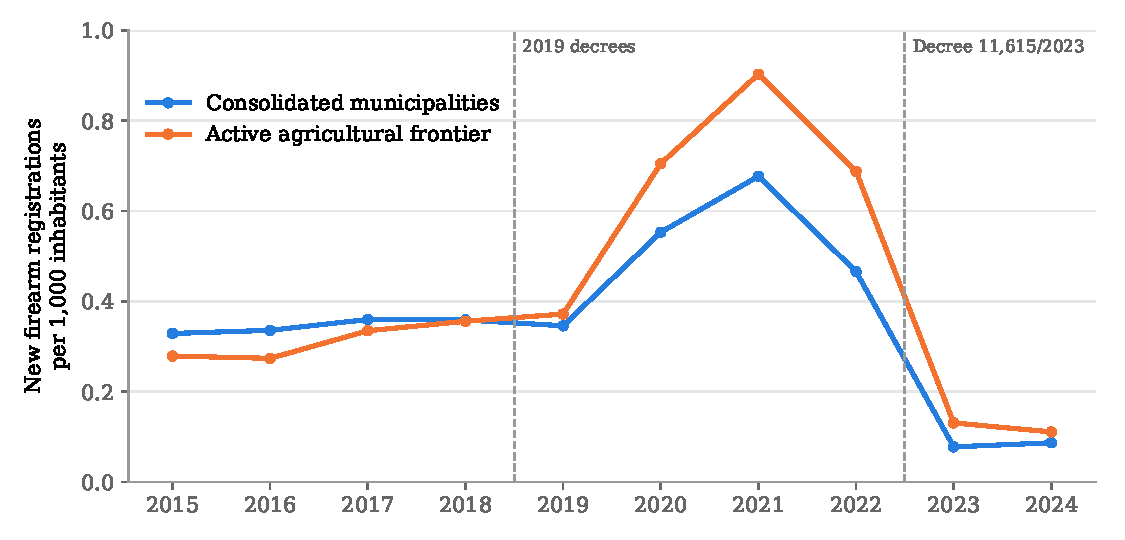
\includegraphics[width=0.78\linewidth]{figs/registros_grupos_en.pdf}
\caption{New civilian firearm registrations per 1,000 inhabitants by territorial group}\label{fig:grupos}
\nota{Aggregate rates by group. Sources: SINARM/Federal Police and IBGE.}
\end{figure}

\begin{figure}[H]
\centering
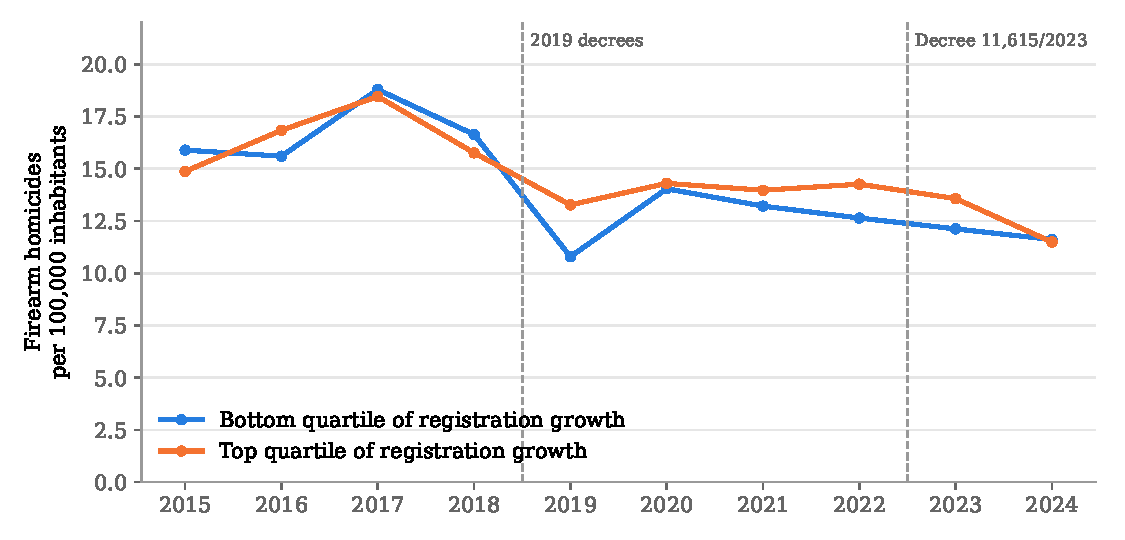
\includegraphics[width=0.78\linewidth]{figs/homicidios_quartis_en.pdf}
\caption{Firearm homicides by quartile of registration growth}\label{fig:quartis}
\nota{Aggregate rates for municipalities in the first and fourth quartiles of $\Delta REG_i$. Sources: SIM/DATASUS, SINARM/Federal Police, and IBGE.}
\end{figure}

\section{Empirical strategy}\label{sec:estrategia}

Because the decrees applied to the whole country at the same time, identification exploits variation across municipalities in the intensity with which the shock materialized. The main specification is
\begin{equation}\label{eq:twfe}
Y_{it} = \alpha_i + \lambda_t + \beta\,(\Delta REG_i \times Post_t) + X_{it}'\gamma + \varepsilon_{it},
\end{equation}
where $Y_{it}$ is the firearm homicide rate in municipality $i$ and year $t$, $\alpha_i$ and $\lambda_t$ are municipality and year fixed effects, $Post_t$ indicates years from 2019 onward, and $X_{it}$ collects the controls. The parameter $\beta$ measures the effect of one additional registration per 1,000 inhabitants on the firearm homicide rate. Regressions are weighted by population, and standard errors are clustered by municipality. We also estimate a fixed-effects Poisson model for death counts, with log population as an offset, and versions that add the interactions $\Delta REG_i \times Post_t \times Frontier_i$ and $\Delta REG_i \times Post2023_t$.

The identifying assumption is that, absent the decrees, municipalities with high and low registration growth would have followed parallel trends in firearm homicides. To assess it, we estimate the event study
\begin{equation}
Y_{it} = \alpha_i + \lambda_t + \sum_{t\neq 2018}\delta_t\,(\Delta REG_i\times \mathbf{1}[\text{year}=t]) + X_{it}'\gamma + \varepsilon_{it}.
\end{equation}
Because the timing with which each municipality absorbed the shock varied, and the two-way fixed effects estimator can be biased under heterogeneous effects \citep{goodmanbacon2021,dechaisemartin2020,sun2021}, we also use the estimator of \citet{callaway2021}. Cohorts are defined by the first year between 2019 and 2021 in which the municipality's annual registration rate reached at least twice its 2015--2018 average, yielding @@c19@@ municipalities in the 2019 cohort, @@c20@@ in the 2020 cohort, and @@c21@@ in the 2021 cohort, with @@c0@@ never-treated municipalities.

Two additional strategies address the main threats to identification. The triple difference
\begin{equation}
Y_{imt} = \alpha_{im} + \lambda_{mt} + \theta_{it} + \beta_{DDD}\,(\Delta REG_i\times FA_m\times Post_t) + \varepsilon_{imt},
\end{equation}
where $m$ indexes the means of the homicide, compares firearm and knife homicides within the same municipality and year and absorbs, through $\theta_{it}$, any local shock that affects violence in general. The SDID estimator of \citet{arkhangelsky2021} reconstructs the pre-treatment trajectory of treated municipalities using unit and time weights and requires a binary treatment with block adoption. Groups are defined in three ways: top versus bottom quartile of $\Delta REG_i$, the 2019 cohort versus never-treated municipalities, and the soy frontier versus consolidated soy producers. SDID standard errors are obtained by a municipality bootstrap with 200 replications.

\section{Results}\label{sec:resultados}

Table~\ref{tab:main} presents the main results. In column (2), which includes controls, $\hat\beta = @@b2@@$, with a standard error of @@b2se@@ (p = @@b2p@@). Moving from the first to the third quartile of exposure (from @@p25@@ to @@p75@@ registrations per 1,000 inhabitants) raises the firearm homicide rate by @@iqr@@ deaths per 100,000, equivalent to @@pctiqr@@\% of the population-weighted mean of @@meanaf@@. The Poisson model indicates a @@pois@@\% increase in firearm homicides for each additional registration per 1,000 inhabitants. The interaction with the agricultural frontier is small and insignificant (@@fint@@; p = @@fintp@@), and the 2023 term shows no reversal through 2024 (@@rev@@; p = @@revp@@). An alternative design that treats the agricultural frontier as the treated group confirms that it received more guns (@@ftreg@@ additional registrations per 1,000 inhabitants per year) but detects no difference in homicides (@@ftaf@@; p = @@ftafp@@), because the binary classification pools municipalities with very different exposures.

\begin{table}[H]
\centering\footnotesize\setlength{\tabcolsep}{4pt}
\caption{Effect of gun registration growth on firearm homicides}\label{tab:main}
\begin{tabular}{lcccccc}
\toprule
 & (1) & (2) & (3) & (4) & (5) & (6) \\
 & TWFE & TWFE & Frontier & Reversal & Poisson & C\&S \\
\midrule
@@tab2@@
\bottomrule
\end{tabular}
\nota{Dependent variable: firearm homicides per 100,000 inhabitants; in column (5), death counts with log population as an offset, and the coefficient is a semi-elasticity. $\Delta REG_i$ is measured in new registrations per 1,000 inhabitants. Column (6) reports the aggregate ATT from the \citet{callaway2021} estimator, with not-yet-treated municipalities as the comparison group. Standard errors clustered by municipality in parentheses. $^{*}$ p$<$0.10; $^{**}$ p$<$0.05; $^{***}$ p$<$0.01.}
\end{table}

The \citet{callaway2021} estimator (column 6) indicates that municipalities that experienced a registration surge record, on average, @@cs@@ additional firearm homicides per 100,000 inhabitants (standard error @@csse@@; 95\% interval from @@cslo@@ to @@cshi@@). The result is nearly identical when never-treated municipalities form the comparison group (@@csnev@@; standard error @@csnevse@@).

Table~\ref{tab:es} and Figures~\ref{fig:es} and \ref{fig:cs} present the dynamics of the effect. In the two-way fixed effects event study, post-2019 coefficients are positive and significant in every year and peak in 2022--2023, when the accumulated stock was largest. The 2015--2017 coefficients are also positive, and the joint test rejects that they are zero (F = @@wF@@; p = @@wp@@), which partly reflects the particularly sharp decline in homicides in 2018 among the most exposed municipalities. In the \citet{callaway2021} estimator, which compares each cohort with its own pre-surge years, the coefficients from $k=-4$ to $k=-1$ are not statistically different from zero, and post-surge effects are positive and increasing.

\begin{table}[H]
\centering\footnotesize\setlength{\tabcolsep}{4pt}
\caption{Dynamic estimates (reference year: 2018)}\label{tab:es}
\begin{tabular}{llccccc}
\toprule
 & & \multicolumn{2}{c}{Firearm homicides} & \multicolumn{2}{c}{Placebo: traffic} & C\&S \\
\cmidrule(lr){3-4}\cmidrule(lr){5-6}
Year & Period & $\hat\delta_t$ & SE & $\hat\delta_t$ & SE & ATT($k$) \\
\midrule
@@tab3@@
\bottomrule
\end{tabular}
\nota{Event study with municipality and year fixed effects, controls, and population weights; standard errors clustered by municipality. The last column reports the \citet{callaway2021} ATT by time $k$ relative to the first registration surge, aligned with the row of the same $k$, with its standard error in parentheses. $^{*}$ p$<$0.10; $^{**}$ p$<$0.05; $^{***}$ p$<$0.01.}
\end{table}

\begin{figure}[H]
\centering
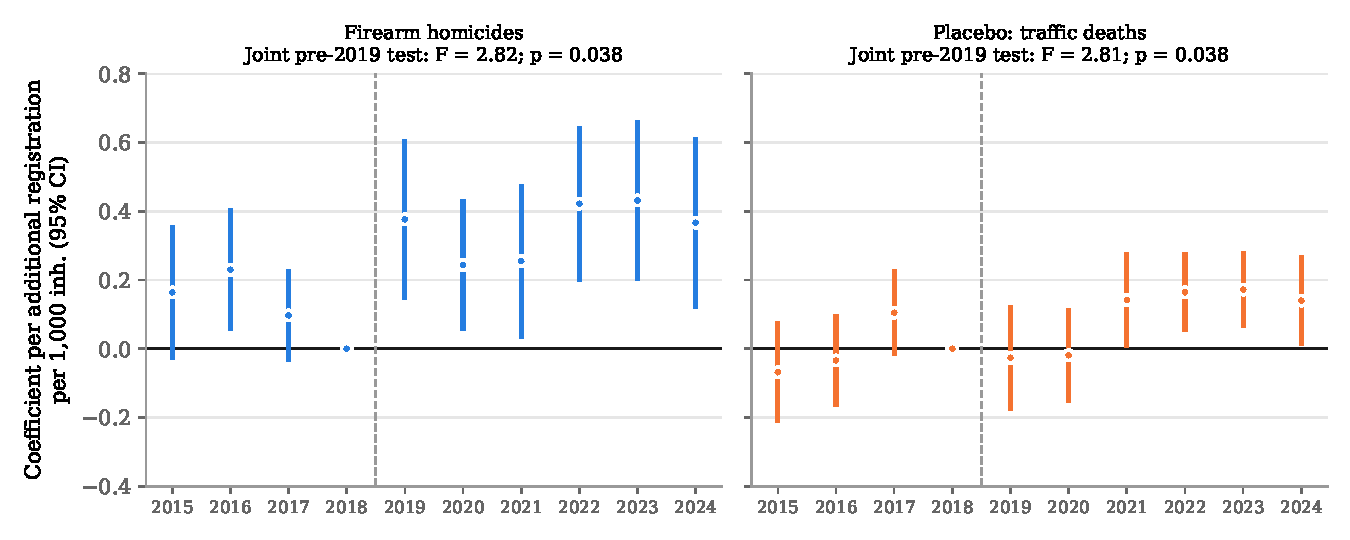
\includegraphics[width=0.95\linewidth]{figs/event_study_en.pdf}
\caption{Event study: dynamic coefficients and 95\% confidence intervals}\label{fig:es}
\nota{Coefficients per additional registration per 1,000 inhabitants; standard errors clustered by municipality.}
\end{figure}

\begin{figure}[H]
\centering
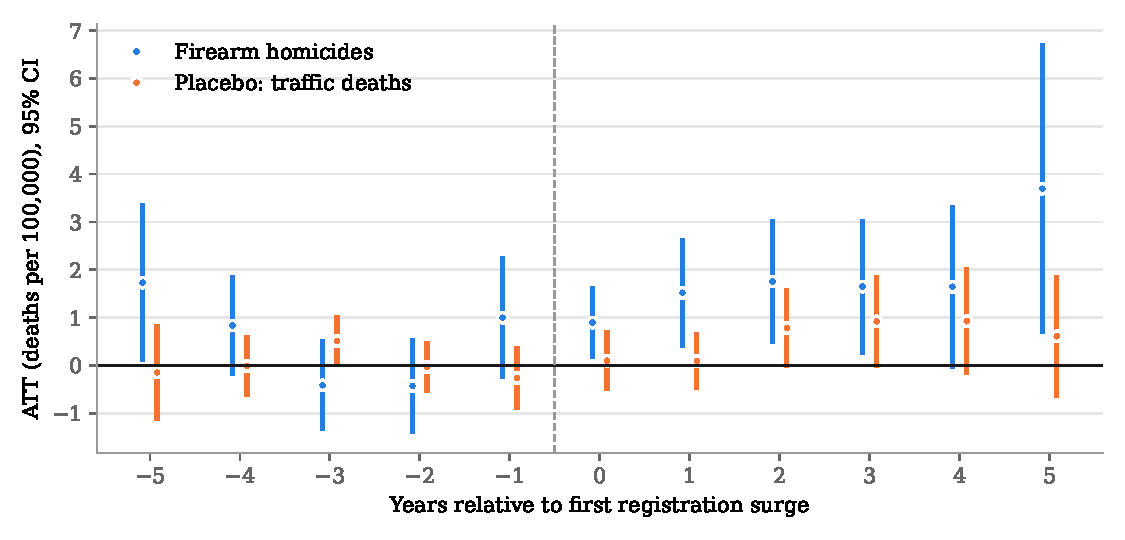
\includegraphics[width=0.75\linewidth]{figs/callaway_santanna_en.pdf}
\caption{Callaway and Sant'Anna: effects by time relative to the first registration surge}\label{fig:cs}
\nota{Not-yet-treated municipalities as the comparison group; population weights; 95\% confidence intervals.}
\end{figure}

\section{Robustness}\label{sec:robustez}

Table~\ref{tab:rob} collects the robustness tests. The triple-difference coefficient is positive and significant (@@ddd@@; p = @@dddp@@), and knife homicides do not respond to registration growth (@@ab@@; p = @@abp@@). The increase in lethality is therefore specific to firearms, which is consistent with the availability channel and rules out explanations based on general trends in local violence. The binary treatment, defined by the top quartile of exposure, yields an effect of @@q4@@ deaths per 100,000. More demanding controls, which include trends specific to pre-2019 registration levels or state-by-year fixed effects, raise the coefficient to about @@ufano@@, which indicates that the result is not driven by regional differences in trends. The effect also holds in municipalities with 20,000 or more inhabitants and within each territorial group.

Two results call for caution. The outcome placebo with traffic deaths is positive and significant in the fixed effects model (@@tr@@; p = @@trp@@), with the effect concentrated in 2021--2024, which suggests a concurrent shock, such as economic and traffic growth in agribusiness municipalities that also registered more guns. In the \citet{callaway2021} estimator, this placebo is not significant (@@cstr@@; standard error @@cstrse@@). The 2017 timing placebo is negative and marginally significant (@@p17@@; p = @@p17p@@), reflecting the same 2018 drop in homicides seen in the event study. Finally, in the 50-municipality sample the effect is not detectable (@@s50@@; p = @@s50p@@), which illustrates the importance of using the universe of municipalities to estimate effects of this magnitude.

\begin{table}[H]
\centering\small
\caption{Robustness tests}\label{tab:rob}
\begin{tabular}{lcccc}
\toprule
Specification & Coefficient & SE & p-value & N \\
\midrule
@@tab4@@
\bottomrule
\end{tabular}
\nota{All regressions include unit and time fixed effects; the triple difference includes municipality-by-means, year-by-means, and municipality-by-year fixed effects. Unless otherwise noted, controls and population weights as in column (2) of Table~\ref{tab:main}. Standard errors clustered by municipality. $^{*}$ p$<$0.10; $^{**}$ p$<$0.05; $^{***}$ p$<$0.01.}
\end{table}

Table~\ref{tab:sdid} and Figure~\ref{fig:sdid} present the SDID estimates. Comparing the 2019 cohort with never-treated municipalities of 20,000 or more inhabitants, the effect is @@c2@@ deaths per 100,000 (standard error @@c2se@@), with an almost perfect pre-treatment fit. Comparing the top and bottom quartiles of exposure, however, the SDID estimate is zero (@@sdb@@; standard error @@sdbse@@) and turns negative when treated municipalities are weighted by population (@@sda2@@; standard error @@sda2se@@). Bottom-quartile municipalities are concentrated in the Northeast, whose homicide dynamics differ from those of the South and Center-West, where top-quartile municipalities are concentrated, and four pre-treatment years provide little information for the synthetic weights to balance such different regions. Placebos with knife homicides and traffic deaths are null. SDID confirms the effect when the comparison is made between similar groups, but not when it contrasts the extremes of the exposure distribution, which calls for caution in interpreting the magnitude.

\begin{table}[H]
\centering\footnotesize\setlength{\tabcolsep}{4pt}
\caption{Synthetic difference-in-differences}\label{tab:sdid}
\begin{tabular}{lccccccc}
\toprule
Treated vs. controls & SDID & SE & DiD & SE & SC & SE & N (T/C) \\
\midrule
@@tab5@@
\bottomrule
\end{tabular}
\nota{Dependent variable: firearm homicides per 100,000 inhabitants. SDID as in \citet{arkhangelsky2021}, with unit and time weights estimated over 2015--2018 and treatment from 2019. DiD uses uniform weights, and SC is synthetic control without time weights. Municipality bootstrap standard errors (200 replications). Q4 and Q1 denote the top and bottom quartiles of $\Delta REG_i$. $^{*}$ p$<$0.10; $^{**}$ p$<$0.05; $^{***}$ p$<$0.01.}
\end{table}

\begin{figure}[H]
\centering
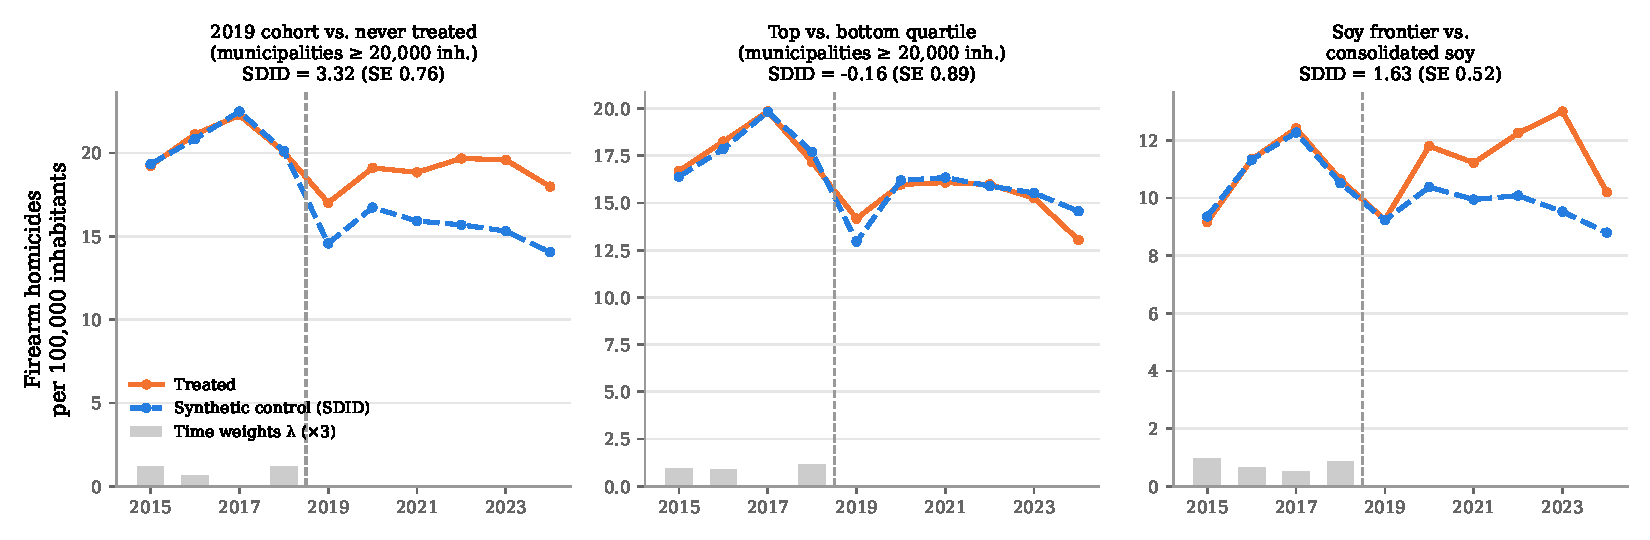
\includegraphics[width=\linewidth]{figs/sdid_en.pdf}
\caption{SDID: trajectories of treated municipalities and synthetic controls}\label{fig:sdid}
\nota{Dashed lines show the SDID synthetic control, and gray bars show the time weights.}
\end{figure}

\section{The soy frontier}\label{sec:soja}

The soy frontier comprises municipalities with at least 1,000 hectares of soy in 2018, a planted area at least 50\% larger than in 2010, and 2015--2018 deforestation above the national median. These criteria identify @@nsoja@@ municipalities, concentrated in Rio Grande do Sul, Mato Grosso, Tocantins, Goiás, Minas Gerais, Santa Catarina, and Maranhão. The comparison groups are the @@ncons@@ consolidated soy producers and the @@nsem@@ municipalities without relevant soy production. Table~\ref{tab:soja} shows that the soy frontier received more guns after 2019 in both comparisons. Against municipalities without soy, the difference-in-differences estimate indicates @@soydid@@ additional homicides per 100,000, but the event study reveals an upward trend before 2019 (joint pre-test p-value of @@soyesp@@), consistent with the spread of violence to the interior of the country.

Estimators that account for this trend confirm the effect. SDID against consolidated soy producers, a comparison that isolates recent expansion among municipalities with the same productive base, yields @@soysd@@ deaths per 100,000 (standard error @@soysdse@@). In the staggered version of the \citet{callaway2021} estimator, in which each frontier municipality enters treatment in the year of its first registration surge (@@sc19@@ municipalities in 2019, @@sc20@@ in 2020, and @@sc21@@ in 2021), the effect is @@soycs@@ deaths per 100,000 (standard error @@soycsse@@; p = @@soycsp@@), with no significant pre-treatment coefficients and similar results under population weights. The triple interaction with the continuous intensity indicates that each additional registration has a larger effect on the soy frontier (@@soyddd@@; p = @@soydddp@@), and knife-homicide placebos are null. On the soy frontier, the effect is therefore about 45\% larger than the national average estimated with the same method. This design, however, does not fully separate gun deregulation from other agribusiness shocks in the period, such as the 2020--2022 commodity price boom; the evidence that the channel operates through guns comes from the larger growth in registrations on the frontier and from the stronger effect per additional registration.

\begin{table}[H]
\centering\footnotesize\setlength{\tabcolsep}{4pt}
\caption{The soy frontier as the treated group}\label{tab:soja}
\begin{tabular}{lcccc}
\toprule
 & \multicolumn{2}{c}{vs. no soy} & \multicolumn{2}{c}{vs. consolidated soy} \\
\cmidrule(lr){2-3}\cmidrule(lr){4-5}
 & Coef. & SE & Coef. & SE \\
\midrule
@@tab6@@
\bottomrule
\end{tabular}
\nota{Soy frontier: at least 1,000 ha of soy in 2018, soy area 50\% larger than in 2010, and 2015--2018 deforestation above the median. DiD with municipality and year fixed effects, controls, and standard errors clustered by municipality; SDID with municipality bootstrap standard errors. In the staggered version of the \citet{callaway2021} estimator, cohorts are defined by the first registration surge, controls are consolidated producers and not-yet-treated municipalities, and frontier municipalities without a surge are excluded. $^{*}$ p$<$0.10; $^{**}$ p$<$0.05; $^{***}$ p$<$0.01. Sources: IBGE/PAM, MapBiomas, SINARM/Federal Police, and SIM/DATASUS.}
\end{table}

\section{Discussion}\label{sec:discussao}

The results are in line with the evidence in \citet{duggan2001}, \citet{cook2006}, and \citet{cerqueira2012}: the expansion of the stock of legal guns in circulation raised firearm homicides through the availability channel, with no visible deterrence in other forms of homicide. The magnitude is moderate. In the \citet{callaway2021} estimator, the effect corresponds to about @@cspct@@\% of the mean rate, and it occurred during a period of national decline in homicides, so that deregulation did not reverse this trend but slowed it in the most exposed municipalities. The absence of reversal through 2024 is consistent with the stock of guns accumulated in 2019--2022 remaining in circulation.

The analysis has limitations. The treatment measure covers civilian guns registered with the Federal Police and excludes CACs, whose registrations are not released by municipality; the estimated effect therefore refers to the expansion of civilian ownership. The joint pre-treatment test of the conventional event study and the traffic-death placebo suggest that part of the association may reflect concurrent local shocks, a concern mitigated, but not eliminated, by the \citet{callaway2021} estimates and by specifications with trend controls. Reverse causality, in which municipalities with rising violence demand more guns, cannot be ruled out; an instrument for pre-2019 local demand for guns would be an improvement. SDID proved sensitive to the comparison group. Finally, the design cannot tell whether the additional homicides were committed with registered guns or with guns diverted to illegal markets, and the deterrence hypothesis regarding property crime could not be tested for lack of municipal data.

\section{Conclusion}\label{sec:conclusao}

This paper has shown that the relaxation of firearm access in Brazil between 2019 and 2022 increased firearm homicides in the municipalities most exposed to the shock. Each additional gun registration per 1,000 inhabitants raised the firearm homicide rate by about @@b2@@ deaths per 100,000 per year, and municipalities that experienced a registration surge recorded, on average, @@cs@@ additional deaths per 100,000. The effect is specific to firearm deaths, larger on the soy frontier, and persistent after the 2023 restrictions. From a policy perspective, the results indicate that the expansion of civilian gun ownership carries a measurable and lasting cost in lives, even after regulatory reversal, because the accumulated stock remains in circulation. Releasing CAC registrations at the municipal level and integrating SINARM and SIGMA would allow more complete evaluations.

\section*{Data and code availability}
All data used in this paper are public. The code used to build the panel and estimate the models is available from the corresponding author upon request.

\bibliographystyle{plainnat}
\bibliography{referencias}

\end{document}
